Avant de développer le concept de réseau virtuel, quelques notions de base de la
théorie des graphes doivent être précisés. Les paragraphes qui suivent ne
constituent nullement un apport nouveau à cette théorie, mais permettent au
lecteur qui n'est pas familier avec cette matière de comprendre les concepts
fondamentaux sur lesquels est basé le réseau virtuel. Ces quelques pages
s'ins\-pirent de l'excellent ouvrage de Minoux et Bartnik\footnote{Minoux M. et
Bartnik G., 1986,``Graphes, Algorithmes, Logiciels``, Dunod informatique. Le
lecteur intéressé lira également avec intérêt l'ouvrage de Gondrand M., Minoux
M.,1979, ``Graphes et Algorithmes``, Eyrolles. Ces deux ouvrages ont été choisis
car ils reprennent et expliquent clairement la plupart des algorithmes
classiques de la théorie des graphes, que ce soit d'un point de vue
méthodologique que d'un point de vue plus informatique. C'est ainsi que la
complexité des algorithmes présentés est à chaque fois calculée, ce qui permet
d'effectuer un choix motivé entre les différents algorithmes, en fonction des
conditions particulières du modèle à développer.}.

\section{Notions de base}

\subsection{Graphe}

Un graphe G = [X, U] est déterminé par:

\begin{itemize}
\item Un ensemble X dont les éléments x $\in$ X sont appelés des sommets ou
des noeuds. N = \#X représente le nombre de noeuds. Le graphe est
dit d'ordre N. Les noeuds sont numérotés i = 1..N.
\item Un ensemble U dont les éléments u $\in$ U sont des couples ordonnés de
noeuds appelés des arcs. Si u = ($x_1,x_2$) est un arc de G, $x_1$
est l'extrémité initiale de u et $x_2$ l'extrémité terminale de u.
Le nombre d'arcs est noté M = \#U.
\end{itemize}

\subsection{Successeurs et pr\'ed\'ecesseurs}

On dit que $x_2$ est un successeur de $x_1$ s'il existe un arc
ayant $x_1$ comme extrémité initiale et $x_2$ comme extrémité
terminale. L'ensemble des successeurs d'un noeud x $\in$ X est noté
$\Gamma_x$.

On dit que $x_2$ est un prédécesseur de $x_1$ s'il existe un arc de
la forme ($x_2,x_1$). L'ensemble des prédécesseurs de x $\in$ X
peut alors être noté $\Gamma_x^{-1}$.

\subsection{Graphe complet}

Un graphe G = [X,U] est dit complet si, pour toute paire de noeuds
($x_1,x_2$), il existe au moins un arc de la forme ($x_1,x_2$) ou
($x_2,x_1$).

Un réseau de transport n'est de ce fait que très rarement, pour ne
pas dire jamais, un graphe complet.

\subsection{Orientation d'un graphe}

A tout arc ($x_1,x_2$) - à tout couple ordonné$(x_1,x_2$) - est
associé le couple non ordonné($x_1,x_2$), appelé l'arête
($x_1,x_2$). Une arête est donc un arc non orienté. Un graphe G =
[X,U] est un graphe non orienté si l'ensemble U est un ensemble
d'arêtes.

Un réseau de transport peut être orienté ou non. En effet, dans un
réseau de type urbain, il est important de tenir compte, par
exemple, des sens uniques. Ce type de réseau est alors orienté. Par
contre, lorsque l'on travaille sur de gros réseaux de transport
nationaux, on peut utiliser un graphe non orienté car chaque arc
peut être parcouru dans les deux sens et au même coût.

Toutefois, bien que le réseau virtuel soit destiné à être utilisé
sur des réseaux de ce second type, il doit être orienté, pour des
raisons qui seront présentées plus loin.

\subsection{Densit\'e d'un graphe}

La densité d'un graphe est le rapport entre le nombre d'arcs
(d'arêtes) d'un graphe et le nombre d'arcs (arêtes) que comporte le
graphe complet ayant le même nombre de noeuds. Ainsi, dans le cas
d'un graphe orienté, la densité est:


$$\frac{M}{N(N-1)} $$

Pour le cas d'un graphe non orienté, la densité s'exprime par:

$$\frac{2M}{N(N-1)} $$

Un réseau de transport (ainsi d'ailleurs que le réseau virtuel qui en découle)
est donc un graphe peu dense. En effet, un noeud n'est jamais lié directement à
tous les autres noeuds. En règle générale, à un noeud sont rattachés 3 ou 4
autres noeuds au maximum. Cette caractéristique peut influencer le choix de
l'algorithme qui sera utilisé pour calculer des chemins.

Ces quelques concepts de base clarifiés, il reste à définir la
notion de réseau multi-modal. Sous cet adjectif se cachent deux
sous-problèmes:


\begin{itemize}
\item  Le choix du mode de transport proprement dit (le camion, le
train, le bateau)
\item Le choix du moyen de transport (le train est-il électrique ou diesel?
Le bateau est-il de 300 tonnes ou de 1000 tonnes?).
\end{itemize}

Si l'on s'en tient aux trois modes de transport terrestres classiques (camions,
trains et bateaux), le réseau multi-modal est composé de trois réseaux
mono-modaux distincts: le réseau routier, le réseau de chemin de fer et le
réseau des voies navigables. Chaque réseau accueille un seul mode de transport,
mais peut accueillir différents moyens de transport. Les différents réseaux sont
inter\-connectés par le biais de gares et/ou ports communs.

Le réseau multi-modal est constitué d'un ensemble de noeuds et un
ensemble d'arêtes. Chaque arête représente une voie utilisable par
un seul mode de trans\-port, mais peut être emprunté par différents
moyens de transport.

Dans le réseau multi-modal tel qu'il a été défini, il est possible de changer de
mode ou de moyen de transport et de prendre plusieurs fois le même mode ou moyen
de transport pour arriver à destination. On peut imaginer charger la marchandise
sur un camion pour utiliser ensuite les voies navigables et reprendre un camion
pour atteindre la destination finale. Le chemin est donc constitué d'un ensemble
de parcours effectués à l'aide d'un seul moyen de transport et de divers
transbordements. Pour chacun de ces parcours, il s'agit de trouver la voie qui
minimise le coût de transport, tout en minimisant les coûts liés aux
transbordements.



\section{Approche intuitive}



Posons les modes de transport R, F et E comme étant respectivement
la
\underline{R}oute, le chemin de \underline{F}er et les voies d'\underline{E}au.


En première analyse, les coûts liés aux frais de chargements et de
transbordements peuvent être considérés comme des poids que l'on
rattache aux noeuds d'un réseau tandis que les coûts liés aux
distances de transport sont rattachés aux arêtes du réseau.

Cependant, il faudrait pouvoir attacher un poids à un noeud de manière
condi\-tion\-nelle. En effet, le coût de chargement ou de transbordement n'est
supporté qu'en cas de chargement ou de transbordement effectif. En d'autres
termes, le passage d'une arête à une autre se déroule souvent sans devoir
changer de mode ou de moyen de transport.

De plus, le poids des noeuds n'est que très rarement unique. Il
suffit pour s'en convaincre d'observer n'importe quel port de
chargement le long du Canal Albert (Belgique). Ce canal peut
supporter des bateaux jusqu'à 9000 tonnes, mais on y rencontre
beaucoup de bateaux plus modestes. Pour un même port, le coût de
chargement d'un petit bateau est évidemment différent de celui d'un
grand.

L'idée de base de la méthode et de l'algorithme proposés est de
créer, à partir d'un réseau réel, un réseau virtuel dans lequel on
crée une arête pour tous les éléments auxquels on affecte un poids.

La solution peut tout d'abord être présentée de manière intuitive en prenant
l'exemple du réseau de voies navigables repris à la figure \ref{f3_1}.

\begin{figure}[htbp]
\centerline{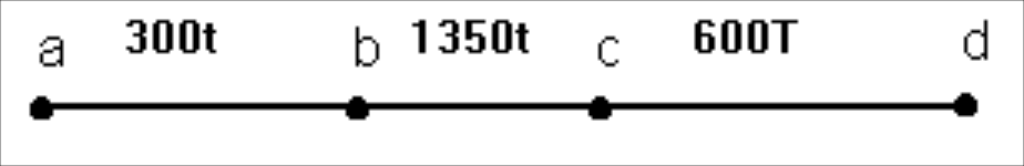
\includegraphics[width=7cm]{f3_1.png}}
\caption{\label{f3_1} R\'eseau hydraulique simple}
\end{figure}


Ce réseau est donc constitué de 4 noeuds et 3 arêtes. Ces dernières
représentent des voies d'eau au gabarit de 300, 1350 et 600 tonnes
respectivement.

Pour passer du noeud a au noeud d, il est possible que le chemin le
moins coûteux consiste à réaliser un transbordement au noeud b pour
passer sur un bateau de 1000 ou de 1350 T, pour repasser ensuite
sur un bateau de 600 tonnes en c.

Une autre possibilité est de passer sur des bateaux de 600 tonnes
dès le noeud b et de continuer ainsi jusqu'en d.

Enfin, un voyage complet rien qu'avec des bateaux de 300 tonnes est
également possible.

Ce réseau, bien que très simple, résume donc très bien le problème
du choix modal.


L'idée de base de la méthode proposée est de créer, à partir d'un réseau réel,
un réseau virtuel dans lequel tous les poids, qu'ils soient liés à des arêtes ou
à des noeuds, sont affectés à des arêtes. La notation utilisée pour les
identificateurs des noeuds dans ce réseau virtuel permetra de connaître
directement le type de coût à associer à chaque arête. Dans l'exemple, le réseau
virtuel dérivé du réseau réel se présente comme dans la figure \ref{f3_2}.

\begin{figure}[htbp]
\centerline{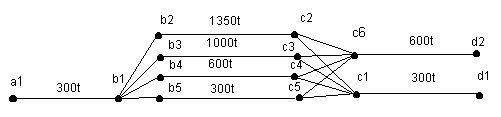
\includegraphics[width=12cm]{f3_2.png}}
\caption{\label{f3_2} R\'eseau virtuel correspondant}
\end{figure}

La solution passe donc par la création d'un ensemble de noeuds nouveaux b1-b5,
c1-c5, d1-d2 et d'un ensemble de nouvelles arêtes reliant ces nouveaux noeuds.

Dans une première étape, toutes les arêtes réelles existantes sont
scindées en arêtes virtuelles en fonction des moyens de transport
utilisables:

\begin{itemize}

\item L'arête (a,b) n'a pas été scindée, car sur un canal de 300 tonnes il
n'est possible de faire passer que des bateaux de 300 tonnes.
\item L'arête (b,c) à été scindée en quatre parties. En effet, sur un canal de
1350 tonnes, il est possible de faire passer des bateaux de 300,
600, 1000 et 1350 tonnes.
\item  L'arête (c,d) est dédoublée, car sur un canal de 600 tonnes il est possible
de faire passer des bateaux de 300 et de 600 tonnes.
\end{itemize}

L'ensemble des arêtes réelles ainsi multiplié, il reste à les
relier grâce à d'autres arêtes virtuelles. Ces dernières
correspondent aux opérations de transbordements.

C'est ainsi que le noeud réel b est représenté dans le réseau
virtuel par 4 noeuds virtuels et 4 arêtes virtuelles. On peut alors
affecter, sur ces arêtes, les coûts des transbordements d'un bateau
de 300 tonnes vers des bateaux de 600, 1000 ou 1350 tonnes. Il
existe également une arête virtuelle qui représente le passage d'un
segment de 300 tonnes vers un autre segment de 300 tonnes. Le poids
de cette arête est nul et correspond au simple passage du bateau
par le noeud (réel) b, sans transbordement.

Le même mécanisme est utilisé pour le noeud réel c. Toutes les combinaisons
modales sont également reprises sous forme d'arêtes et de noeuds virtuels. Deux
arêtes de poids nuls sont créées pour des bateaux de 600 et de 300 tonnes ``qui
ne font que passer``.

De cette manière, le réseau multi-modal est représenté par un réseau mono-modal
sur lequel chaque arête a un poids unique représentant soit le coût du
déplacement sur une certaine distance, soit le coût d'un éventuel
transbordement. Lorsqu'un coût aura été affecté à chaque arête, le chemin de
coût minimum peut être calculé en utilisant un algorithme tel que celui de
Johnson. La solution ainsi trouvée est une solution exacte tenant compte de tous
les choix possibles et non pas une heuristique qui donnerait une solution
approchée.

\section{ D\'eveloppement syst\'ematique}

Il reste maintenant à modéliser ce concept de réseau virtuel et à
écrire l'algorithme qui permet de générer un réseau virtuel à
partir d'un réseau réel. Afin de rendre la lecture des quelques
pages qui suivent plus facile, les différentes étapes de la mise au
point de l'algorithme seront illustrées sur la base d'un exemple
simple de réseau.


\subsection{M\'ethode g\'en\'erale}\label{Methode generale}


Soit le réseau réel G = [X,U] de la figure \ref{f3_3}.Ce réseau est composé de 4
noeuds (\#X = N = 4) a, b, c et d et de 5 arêtes (\#U = M = 5) numérotées de 1 à
5.


\begin{figure}[htbp]
\centerline{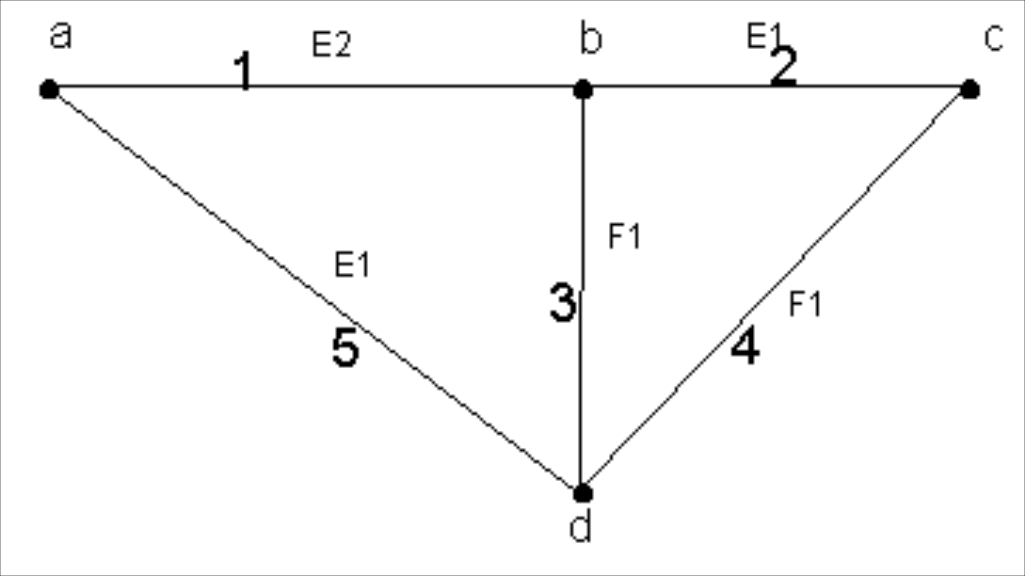
\includegraphics[width=8cm]{f3_3.png}}
\caption{\label{f3_3} R\'eseau multi-modal}
\end{figure}

Deux modes de transport sont présents sur le réseau: les voies
navigables E(au) et le chemin de fer F(er). En ce qui concerne les
voies navigables, il y a des canaux de deux gabarits différents (E1
et E2), représentant respectivement des canaux de 300 et de 600
tonnes. Sur les arêtes de type E2, il est donc possible de faire
passer des bateaux de type E1 et E2. Il n'y a qu'un seul type de
train possible, F1 (train diesel). Il est important de donner une
notation cohérente aux moyens de transport. En effet, si un arc
supporte, par exemple, des convois de type E4, il faut qu'il puisse
laisser passer des convois de types E1, E2 et E3. C'est pour cette
raison que le train diesel est noté F1 et le train électrique F2,
dans la mesure où une locomotive diesel peut rouler sur des lignes
électrifiées, l'inverse n'étant pas vrai.

Le réseau peut se représenter dans le tableau \ref{tab3_1}.

\begin{table}[htbp]
\begin{center}
\begin{tabular}{cccc}
\hline
Numéro d'arête & Noeud 1 & Noeud 2 & Type de voie\\
\hline
1 & a & b & E2\\

2 & b & c & E1\\

3 & b & d & F1\\

4 & d & c & F1\\

5 & a & d & E1\\
\hline
\end{tabular}
\caption{\label{tab3_1} Notation du r\'eseau r\'ell }
\end{center}
\end{table}


La première étape de la méthode de création du réseau virtuel
consiste à passer en revue l'ensemble des arêtes U en créant
($\rightarrow$) pour chaque arête réelle j $\in$ U, autant d'arêtes
virtuelles $\bar u_j^{tm}$ qu'il y a de moyens de transport m
possibles associés au mode de transport t sur cette arête:

$$\forall _{j\in U} \forall _m u_j \rightarrow \bar u_j^{tm}$$

Chaque arête viruelle $\bar u_j^{tm}$ a pour extrémité deux noeuds
virtuels $\bar x_o^{jtm}$ et  $\bar x_d^{jtm}$ affectés d'un
identifiant codé en quatre parties de la manière suivante:

\begin{itemize}

\item L'identificateur du noeud réel i dont il est issu,

\item  L'identificateur de l'arête réelle j qui vient d'être multipliée
(dans le cas où plusieurs moyens de transport sont possibles sur cette arête),

\item  L'identificateur du mode de transport t sur l'arête réelle j,

\item L'identificateur du moyen de transport  m possible sur la nouvelle arête
virtuelle issue de l'arête réelle j.
\end{itemize}

Un noeud virtuel peut donc bien se noter  $\bar x_i^{jtm}$.

Comme chaque arête réelle a une origine o et une destination d, cette arête
réelle génèrera les arêtes virtuelles $\bar u_j^{tm}=(\bar x_o^{jtm},\bar
x_o^{jtm})$ (voir tableau \ref{tab3_2}).

\begin{table}[htbp]
\begin{center}
\begin{tabular}{ccc}
\hline
Arêtes réelles & Arêtes virt. Origine & Arête virt. Destination\\

\hline
1 & a1E2 & b1E2\\

  & a1E1 & b1E1\\

2 & b2E1 & c2E1\\

3 & b3F1 & d3F1\\

4 & d4F1 & c4F1\\

5 & a5E1 & d5E1\\
\hline
\end{tabular}
\caption{\label{tab3_2} Ar\^etes de d\'eplacement}
\end{center}
\end{table}

\begin{figure}[htbp]
\centerline{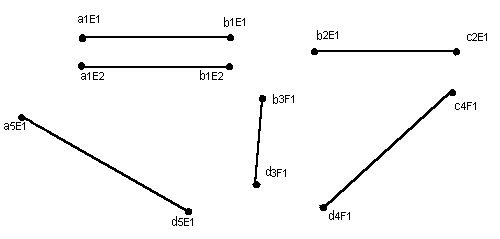
\includegraphics[width=12cm]{f3_4.png}}
\caption{\label{f3_4} S\'eparation des moyens de transport}
\end{figure}



A partir de ce premier résultat (figure \ref{f3_4}), il faut générer l'ensemble
des arêtes qui représentent les transbordements possibles. Cette opération se
fait pour tous les noeuds réels. Or, dans la première phase, tous les noeuds
réels viennent d'être remplacés par un ensemble de noeuds virtuels.

$$\forall_{i \in X}, X_j \rightarrow \bigcup \bar x_i^{jtm} $$

Tous les noeuds virtuels qui font référence au même noeud réel
doivent être reliés entre eux pour représenter l'ensemble des
transbordements possibles
\footnote{Il est évident que ce n'est pas parce que deux arêtes se touchent
qu'un transbordement est possible au noeud qui relie ces deux
arêtes. Ce cas sera considéré plus loin.}.



$$\forall_k \forall_{k'}\rightarrow (\bar x_i^{ktm}, \bar x_i^{k't'm'})$$


Ce qui donne le tableau \ref{tab3_3} pour le noeud réel b (figure \ref{f3_5}):

\begin{table}[htbp]
\begin{center}
\begin{tabular}{ccc}
\hline
Arêtes réelles & Arêtes virt. Origine & Arête virt. Destination\\

\hline
b & b1E1 & b1E2\\

  & b1E1 & b2E1\\

  & b1E2 & b2E1\\

  & b1E1 & b3F1\\

  & b1E2 & b3F1\\

  & b2E1 & b3F1\\

\hline
\end{tabular}
\caption{\label{tab3_3} Ar\^etes de transbordement}
\end{center}
\end{table}

\begin{figure}[htbp]
\centerline{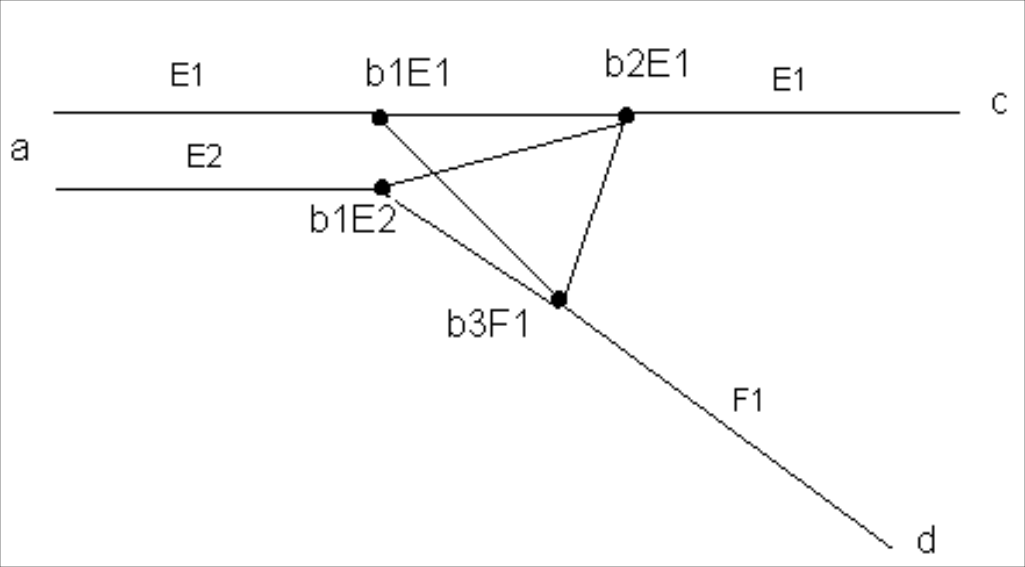
\includegraphics[width=8cm]{f3_5.png}}
\caption{\label{f3_5} Transbordements}
\end{figure}





A ce stade, deux types d'arêtes virtuelles sont à considérer:

\begin{itemize}
\item Celles qui représentent une distance à parcourir. Ces arêtes
représentent les arêtes du réseau réel, éventuellement multipliées
si plusieurs moyens de transport sont possibles. Une telle arête a
comme extrémité deux noeuds virtuels provenant de deux noeuds réels
différents.
\item Les autres arêtes virtuelles représentent tous les transbordements
possibles. Chaque noeud virtuel est ainsi relié à tous les autres
noeuds virtuels dont l'identificateur fait référence au même noeud
réel, en excluant toutefois ceux qui sont issus de la même arête
réelle.
\end{itemize}

Dans le tableau \ref{tab3_4}, les deux dernières colonnes reprennent les coûts
encourus sur chaque arête virtuelle. Lorsqu'il s'agit d'une arête issue
directement du réseau réel, il s'agit d'un déplacement entre deux noeuds et le
poids est fonction de la distance parcourue. Un coût nul dans la colonne
 ``transbordement`` représente un bateau ``qui ne fait que passer
\footnote{Dans certains cas, ce coût n'est pas réellement nul car ce type
d'arcs virtuels peut très bien servir  à représenter un coût lié,
par exemple, au passage d'une frontière ou au péage sur une
autoroute.}``. Les coûts de type ``E2$\rightarrow$E1`` représentent
les coûts liés aux transbordements, ici le passage de bateaux de
600 tonnes à des bateaux de 300 tonnes. On ne peut avoir un coût à
la fois dans la colonne ``transbordement`` et ``déplacement``.


\begin{table}[htbp]
\begin{center}
\begin{tabular}{cccc}
\hline
Origine & Destination & Coût transbordement & Coût déplacement\\
\hline
a1E1 & b1E1 & -                   & Coût = $f(distance)$\\

a1E2 & b1E2 & -                   & Coût = $f(distance)$\\

b1E2 & b1E1 & E2$ \rightarrow$ E1 & -\\

b1E1 & b2E1 & 0 & -\\ b1E2 & b2E1 & E2$ \rightarrow$ E1 & -\\

b1E1 & b3F1 & E1$ \rightarrow$ F1 & -

\\ b1E2 & b3F1 & E2$ \rightarrow$ F1 & -

\\b2E1 & b3F1 & E1$ \rightarrow$ F1 & -\\ b2E1 & c2E1 & - & Coût = $f(distance)$\\

b3F1 & d3F1 & -                   & Coût = $f(distance)$\\
\hline
\end{tabular}
\caption{\label{tab3_4} Op\'erations possibles autour du noeud r\'eel b}
\end{center}
\end{table}


Si la même opération est répétée pour tous les noeuds réels, le réseau virtuel
ressemblera à la figure \ref{f3_6}.

\begin{figure}[htbp]
\centerline{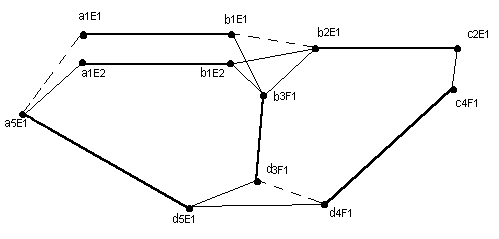
\includegraphics[width=12cm]{f3_6.png}}
\caption{\label{f3_6} R\'eseau virtuel partiel}
\end{figure}


Dans ce réseau, les arêtes en gras représentent les arêtes du réseau réel,
éven\-tu\-el\-le\-ment scindées. Les arêtes en pointillés représentent les
arêtes virtuelles de coût nul. Enfin, les transbordements sont représentés par
des traits pleins non gras.

Cette méthode peut se traduire par l'algorithme présenté à la figure \ref{algo1}
(Le symbole \# est utilisé pour la concaténation d'identificateurs).


\begin{center}
\begin{figure}[htbp]
\center
\fbox{
\begin{minipage}{20cm}
\center
\begin{tabbing}
xxxxx\=xxxxx\=xxxxx\=xxxxx\=xxxxx\=xxxxx\=xxxxx\=xxxxx\=xxxxx\=xxxxx\=\kill
\bf {DEFINIR} \\
tab1, tab2: vecteurs de noeuds virtuels\\ t1, t2 : index dans ces
vecteurs\\
\\

\bf {ENTREE}\\
t1 $\leftarrow$ 1\\
\bf {POUR } j = 1 $\rightarrow$ mode $\leftarrow$ \it{mode de transport sur arête j}\\
\> k $\leftarrow$ \it {nombre de moyens de transport sur arête j}\\
\> \bf {POUR} l = 1 $\rightarrow$ k\\
\> \>  n1 $\leftarrow$\it {noeud d'origine de l'arête j}\\
\> \> n2 $\leftarrow$\it {noeud de destination de l'arête j}\\
\> \> noeud1 $\leftarrow$ n1\#j\#mode\#k\\
\> \>  noeud2 $\leftarrow$ n2\#j\#mode\#k\\
\> \>  \it { Sauver arête(noeud1, noeud2)}\\
\> \> tab[t1] $\leftarrow$ noeud1\\
\> \>  tab[t+1] $\leftarrow$ noeud2\\
\> \> t1 $\leftarrow$ t1 + 2\\
\>  \bf {FIN POUR} i\\
\bf {FIN POUR} j\\
\\
\bf {POUR} k = 1 $\rightarrow$ N\\
\> tab2[ ] $\leftarrow$ \it{partie de tab1[ ] issue du noeud k}\\
\> t2 $\leftarrow$ \it {taille de tab2[ ]}\\
\> \bf{POUR}  i = 1 $\rightarrow$ t2\\
\> \> \bf{POUR} j = i+1 $\rightarrow$ t2\\
\> \> \> \it{Sauver arête(tab2[i], tab2[j])}\\
\> \> \bf{FIN POUR} j\\
\> \bf {FIN POUR} i\\
\bf {FIN POUR} k\\
\bf {SORTIE}\\
\end{tabbing}
\end{minipage}
}
\caption{\label{algo1} Algorithme de base}
\end{figure}
\end{center}



\subsection{Les noeuds d'entr\'ee}


Il reste cependant un problème: s'il est possible de voyager dans
le réseau virtuel, il n'est pas possible d'y entrer ou d'en sortir!
En effet, l'utilisateur final demande de rechercher un chemin entre
les noeuds réels a et b et non pas entre les noeuds virtuels axxx
et bxxx.  De plus, entrer et sortir du réseau a un coût puisqu'il
faut charger et décharger la marchandise.

La solution vient encore des arêtes et des noeuds virtuels. En
effet, si on reprend l'exemple du noeud b, il suffit de créer un
nouveau noeud virtuel b000 et de le relier à tous les autres noeuds
virtuels générés pour ce noeud réel. Toutes ces nouvelles arêtes
représentent les coûts de chargement ou de déchargement de la
marchandise.

$$x_i \rightarrow \bar x_i^{000}$$

$$\forall_i \forall_{ktm} \rightarrow (\bar x_i^{ktm}, \bar x_i^{000})$$


Ce qui donne le tableau \ref{tab3_5} et la figure \ref{f3_7} pour le noeud b:

\begin{figure}[htbp]
\centerline{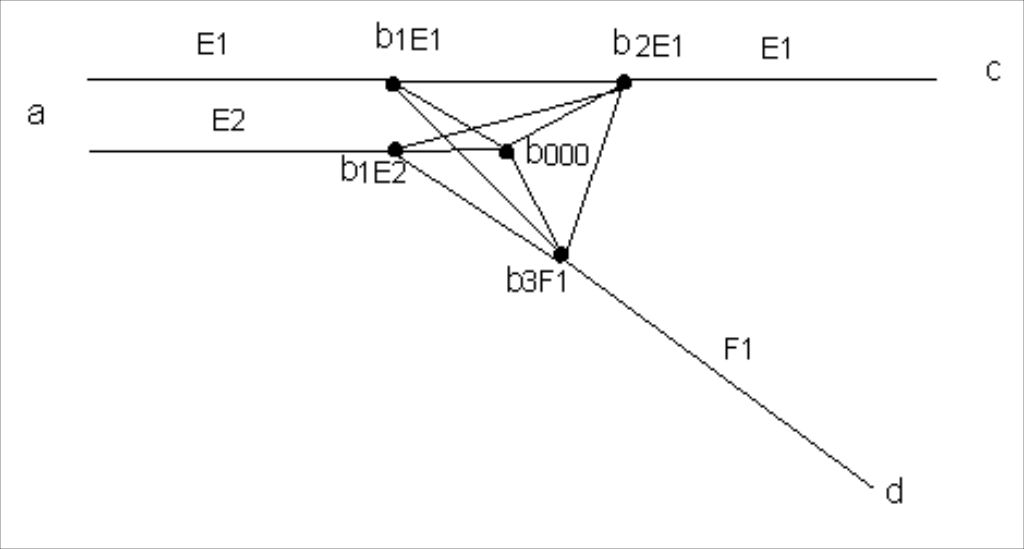
\includegraphics[width=12cm]{f3_7.png}}
\caption{\label{f3_7} Chargements/D\'echargements}
\end{figure}

\begin{table}[htbp]
\begin{center}
\begin{tabular}{ccc}
\hline
Origine & Destination & Coût\\
\hline
b000 & b1E1 & 0 $\rightarrow$ E1\\

b000 & b1E2 & 0 $\rightarrow$ E2\\

b000 & b2E1 & 0 $\rightarrow$ E1\\

b000 & b3F1 & 0 $\rightarrow$ F1\\
\hline
\end{tabular}
\caption{\label{tab3_5} Ar\^etes virtuelles de (d\'e)chargement}
\end{center}
\end{table}

Dans le tableau \ref{tab3_5}, le coût représente le chargement initial de la marchandise ou son déchargement final.

L'algorithme présenté plus haut doit être modifié pour tenir compte de ces
nouveaux noeuds virtuels et arêtes virtuelles (voir figure \ref{algo2}).

\begin{center}
\begin{figure}[htbp]
\center
\fbox{
\begin{minipage}{20cm}
\begin{tabbing}
xxxxx\=xxxxx\=xxxxx\=xxxxx\=xxxxx\=xxxxx\=xxxxx\=xxxxx\=xxxxx\=xxxxx\=\kill
\bf {DEFINIR} \\
tab1, tab2: vecteurs de noeuds virtuels\\ t1, t2 : index dans ces
vecteurs\\
\\

\bf {ENTREE}\\
t1 $\leftarrow$ 1\\
\bf {POUR } j = 1 $\rightarrow$ mode $\leftarrow$ \it{mode de transport sur arête j}\\
\> k $\leftarrow$ \it {nombre de moyens de transport sur arête j}\\
\> \bf {POUR} l = 1 $\rightarrow$ k\\
\> \>  n1 $\leftarrow$\it {noeud d'origine de l'arête j}\\
\> \> n2 $\leftarrow$\it {noeud de destination de l'arête j}\\
\> \> noeud1 $\leftarrow$ n1\#j\#mode\#k\\
\> \>  noeud2 $\leftarrow$ n2\#j\#mode\#k\\
\> \>  \it { Sauver arête(noeud1, noeud2)}\\
\> \> tab[t1] $\leftarrow$ noeud1\\
\> \>  tab[t+1] $\leftarrow$ noeud2\\
\> \> t1 $\leftarrow$ t1 + 2\\
\>  \bf {FIN POUR} i\\
\bf {FIN POUR} j\\
\\
\bf {POUR} k = 1 $\rightarrow$ N\\
\> tab2[ ] $\leftarrow$ \it{partie de tab1[ ] issue du noeud k}\\
\> t2 $\leftarrow$ \it {taille de tab2[ ]}\\
\> \bf{POUR}  i = 1 $\rightarrow$ t2\\
\> \> \bf{POUR} j = i+1 $\rightarrow$ t2\\
\> \> \> \it{Sauver arête(tab2[i], tab2[j])}\\
\> \> \bf{FIN POUR} j\\
\> \bf {FIN POUR} i\\
\\
\> \bf{POUR} i = 1 $\rightarrow$ t2\\
\> \> noeud $\leftarrow$ \it{partie ``noeud'' de tab2[i]\#000}\\
\> \> \it{Sauver arête(noeud, tab2[i])}\\
\> \bf{FIN POUR} i\\
\bf {FIN POUR} k\\
\bf {SORTIE}\\
\end{tabbing}
\end{minipage}
}
\caption{\label{algo2} Introduction des (d\'e)chargements}
\end{figure}
\end{center}


\subsection{Les noeuds de simple passage}

A ce stade, la méthode est difficilement applicable à un réseau réel dans la
mesure où un tel réseau comprend toute une série de noeuds qui ne sont pas des
points de chargement/déchargement. Le réseau routier comprend une multitude de
carrefours qui sont autant de noeuds mais qui ne sont pas des points de
chargement. De la même manière, le réseau de chemin de fer comprend un ensemble
de gares qui sont exclusivement réservées aux passagers et dans les\-quelles
tout transbordement de marchandise est impossible.

Pour ces noeuds, il ne faut pas générer d'arêtes virtuelles qui
correspondent à des transbordements.

Dans l'exemple de la figure \ref{f3_8}, le noeud b représente un point d'
intersection entre une voie d'eau de 600 tonnes (E2) et une autre de 300 tonnes
(E1).


\begin{figure}[htbp]
\centerline{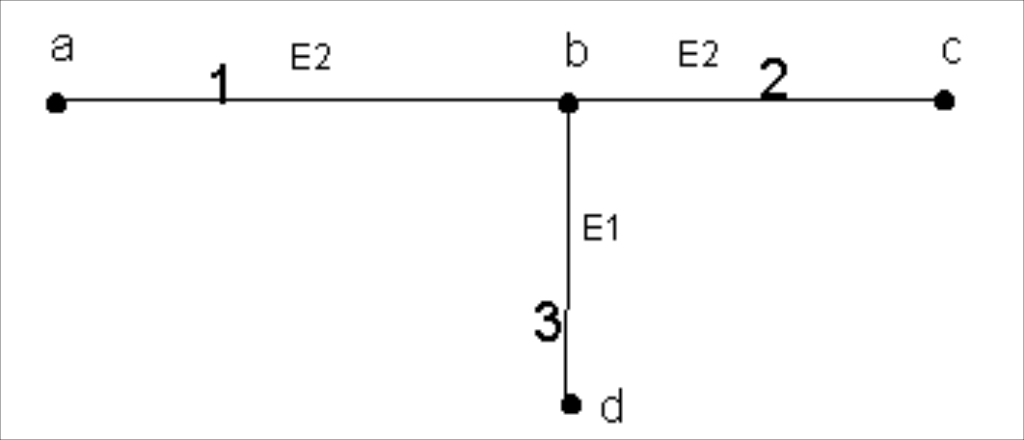
\includegraphics[width=8cm]{f3_8.png}}
\caption{\label{f3_8} Intersection de deux voies d'eau}
\end{figure}

Les voies de type E2 supportent également des convois de type E1.
Un bateau de 600 tonnes provenant du segment 1 peut donc continuer
vers le segment 2, mais pas vers le segment 3.

La méthode expliquée précédemment conduit donc à la création des noeuds
représentés dans le tableau \ref{tab3_6}:

\begin{table}
\begin{center}
\begin{tabular}{ccccc}
\hline
Noeud réel & Arête réelle & Mode & Moyen & Noeud\\
\hline
b & 1 & E & 1 & b1E1\\

b & 1 & E & 2 & b1E2\\

b & 2 & E & 1 & b2E1\\

b & 2 & E & 2 & b2E2\\

b & 3 & E & 1 & b3E1\\
\hline
\end{tabular}
\caption{\label{tab3_6} Ar\^etes de simple transit}
\end{center}
\end{table}




Il reste maintenant à générer les arêtes virtuelles. De nouveau, il
s'agit de relier les noeuds reliés par une arête qui représente une
distance à parcourir, ainsi que chaque noeud virtuel à tous les
autres générés à partir du même noeud réel en excluant les liens
entre les noeuds virtuels dont l' identificateur fait référence à
la même arête réelle. Mais cette fois, seuls les noeuds faisant
référence à la même combinaison mode-moyen de transport (t = t' et
m = m') peuvent être reliés entre eux. C'est ainsi que l'on va
relier b1E2 et b2E2, mais pas b1E2 et b3E1 (cette dernière liaison
signifierait un transbordement d'un bateau de 600 tonnes vers un
bateau de 300 tonnes ou inversement). En d'autres mots, il s'agit
de créer uniquement toutes les arêtes virtuelles de coût ``nul''.
De plus, ces noeuds de ``passage`` n'étant pas des points d'entrée
ou de sortie du réseau, il ne faut pas créer le noeud b000 et les
arêtes virtuelles qui en découlent.


\begin{center}
Si (i = transbordement) ou (t = t' et m = m') $\rightarrow
\forall_k \forall_{l} \rightarrow(\bar x_i^{ktm},
\bar x_i^{lt'm'})$\\
Si i est un noeud de transbordement $\rightarrow \forall_i
\forall_{ktm}
\rightarrow (\bar x_i^{ktm}, \bar x_i^{000})$
\end{center}

Ce qui mène à la création de l'ensemble des arêtes reprises dans le tableau
\ref{tab3_7} (voir également la figure \ref{f3_9}):

\begin{table}[htbp]
\begin{center}
\begin{tabular}{cccc}
\hline

Origine & Destination & Coût transbordement & Coût déplacement\\
\hline
a1E1 & b1E1 & - & $f(distance)$\\

a1E2 & b1E2 & - & $f(distance)$\\

b2E1 & c2E1 & - & $f(distance)$\\

b2E2 & c2E2 & - & $f(distance)$\\

b3E1 & d3E1 & - & $f(distance)$\\

b1E1 & b2E1 & 0 & -\\

b1E1 & b3E1 & 0 & -\\

b2E1 & b3E1 & 0 & -\\

b1E2 & b3E2 & 0 & -\\
\hline
\end{tabular}
\caption{\label{tab3_7} R\'eseau virtuel \`a l'intersection}
\end{center}
\end{table}

\begin{figure}[htbp]
\centerline{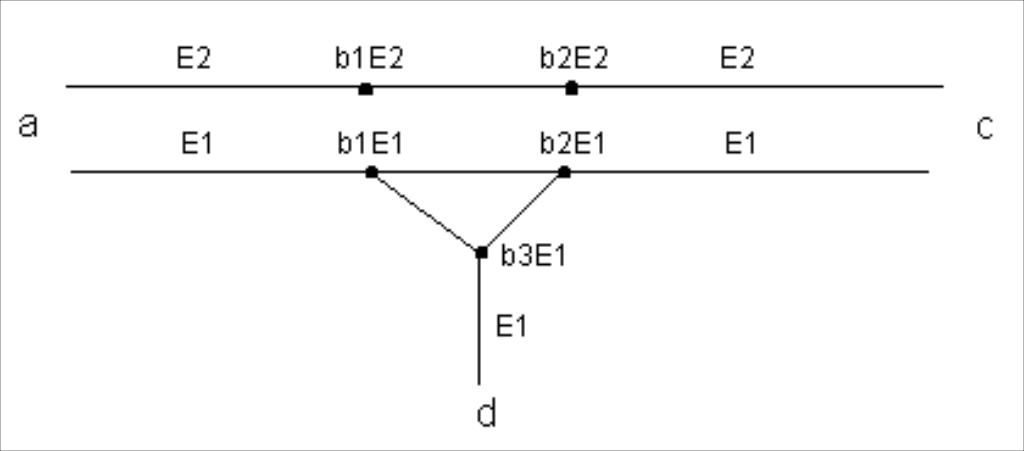
\includegraphics[width=10cm]{f3_9.png}}
\caption{\label{f3_9} R\'eseau virtuel \`a l'intersection}
\end{figure}



La méthode diffère donc selon que le noeud soit un lieu de chargement /
dé\-char\-ge\-ment / transbordement ou un simple lieu de passage. Les noeuds du
graphe doivent dès lors être marqués comme faisant partie d'une de ces deux
catégories.

Ce traitement différencié (voir figure \ref{algo3}) a une conséquence très
intéressante. En effet, du fait que les noeuds ``de passage`` génèrent moins
d'arêtes virtuelles, le réseau virtuel lui-même sera constitué de nettement
moins d'arêtes que celui généré par l'algorithme de base, ce qui accélère le
temps de traitement.


\begin{center}
\begin{figure}[htbp]
\center
\fbox{
\begin{minipage}{20cm}
\begin{tabbing}
xxxxx\=xxxxx\=xxxxx\=xxxxx\=xxxxx\=xxxxx\=xxxxx\=xxxxx\=xxxxx\=xxxxx\=\kill
\bf {DEFINIR} \\
tab1, tab2: vecteurs de noeuds virtuels\\ t1, t2 : index dans ces
vecteurs\\
\\

\bf {ENTREE}\\
t1 $\leftarrow$ 1\\
\bf {POUR } j = 1 $\rightarrow$ mode $\leftarrow$ \it{mode de transport sur arête j}\\
\> k $\leftarrow$ \it {nombre de moyens de transport sur arête j}\\
\> \bf {POUR} l = 1 $\rightarrow$ k\\
\> \>  n1 $\leftarrow$\it {noeud d'origine de l'arête j}\\
\> \> n2 $\leftarrow$\it {noeud de destination de l'arête j}\\
\> \> noeud1 $\leftarrow$ n1\#j\#mode\#k\\
\> \>  noeud2 $\leftarrow$ n2\#j\#mode\#k\\
\> \>  \it { Sauver arête(noeud1, noeud2)}\\
\> \> tab[t1] $\leftarrow$ noeud1\\
\> \>  tab[t+1] $\leftarrow$ noeud2\\
\> \> t1 $\leftarrow$ t1 + 2\\
\>  \bf {FIN POUR} i\\
\bf {FIN POUR} j\\
\\
\bf {POUR} k = 1 $\rightarrow$ N\\
\> tab2[ ] $\leftarrow$ \it{partie de tab1[ ] issue du noeud k}\\
\> t2 $\leftarrow$ \it {taille de tab2[ ]}\\
\> \bf{POUR}  i = 1 $\rightarrow$ t2\\
\> \> \bf{POUR} j = i+1 $\rightarrow$ t2\\
\> \> \> \bf{SI} \it{pas lieu de transbordement}\\
\> \> \> \> \bf{ET} \it{partie ``mode'' de tab2[i] = partie ``mode'' de tab2[j]}\\
\> \> \> \> \bf{ET} \it{partie ``moyen'' de tab2[i] = partie ``moyen'' de tab2[j])}\\
\> \> \> \bf{OU} \it{lieu de transbordement}\\
\> \> \> \> \> \bf{ALORS} \it {Sauver arête(tab2[i], tab2[j])}\\
\> \> \> \bf{FIN SI}\\
\> \> \bf{FIN POUR} j\\
\> \bf {FIN POUR} i\\
\\
\> \bf{POUR} i = 1 $\rightarrow$ t2\\
\> \> \bf{SI} \it{lieu de transobrdement} \bf{ALORS}\\
\> \> \> noeud $\leftarrow$ \it{partie ``noeud'' de tab2[i]\#000}\\
\> \> \> \it{Sauver arête(noeud, tab2[i])}\\
\> \> \bf{FIN SI}\\
\> \bf{FIN POUR} i\\
\bf {FIN POUR} k\\
\bf {SORTIE}\\
\end{tabbing}
\end{minipage}
}
\caption{\label{algo3} Introduction des "simples passages"}
\end{figure}
\end{center}

\subsection{Orientation du r\'eseau virtuel}

La méthode proposée ici mène à la génération d'un réseau virtuel
non orienté. Etant donné que chaque arête doit être pondérée par un
poids unique (un coût), l'utilisation d'un graphe non orienté pose
le problème de l'égalité des coûts lorsque l'on se déplace de
l'origine vers la destination ou de la destination vers l'origine.

Cette hypothèse ne peut pas être justifiée sur un réseau de transport de
marchan\-di\-ses. En effet, certains coûts sont fonction du sens sur l'arc.
C'est le cas par exemple des chargements et des déchargements: on sait par
exepérience qu'il est souvent plus long de décharger que de charger.

Dans la pratique, l'algorithme du réseau virtuel génèrera des arcs
orientés, ce qui permet d'affecter des coûts différents selon le
sens de l'arête virtuelle. Afin de n'avoir qu'un et un seul arc entre deux noeuds virtuels (et donc d'éviter des ``boucles'' dans la recherche du chemin le moins coûteux), chacun de ces noeuds sera ``dédoublé'' en les faisant précéder par un signe positif ou négatif. 

En utilisant la notation proposée dans la section \ref{Methode generale}, le réseau virtuel généré autours du noeud b et illustré par la figure \ref{f3_7} peut être représenté comme dans la figure \ref{f3_7b}.

\begin{figure}[htbp]
\centerline{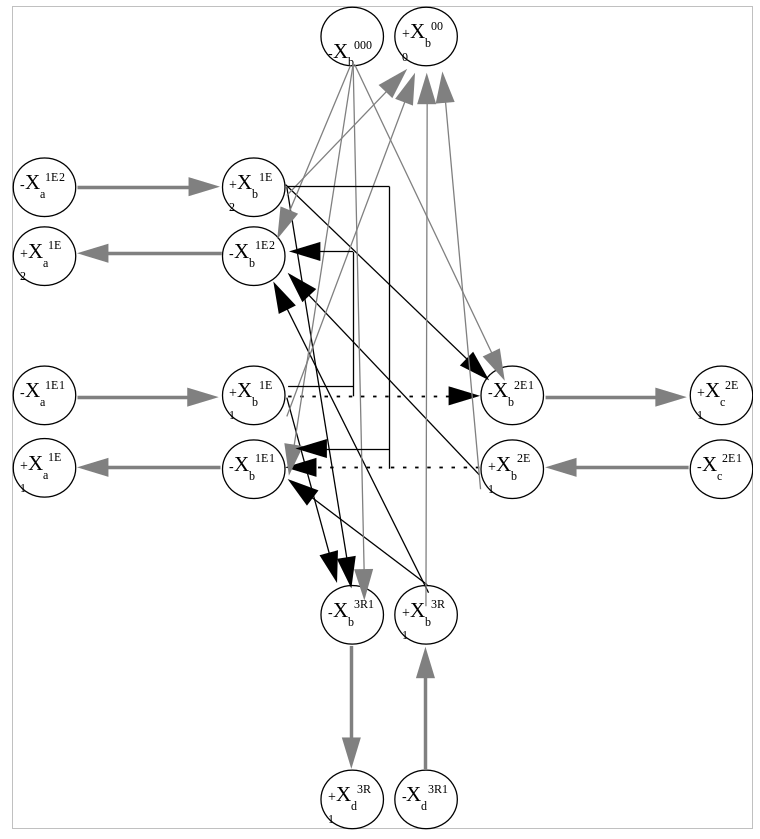
\includegraphics[width=10cm]{f3_7b.png}}
\caption{\label{f3_7b} R\'eseau virtuel orient\'e}
\end{figure}

\subsection{Contr\^ole de la g\'en\'eration du r\'eseau virtuel}


Le réseau virtuel, tel qu'il a été défini jusqu'à présent est le
résultat d'une procédure automatique. Or, cette façon de travailler
présente certaines limites dans la mesure où on peut avoir des
possibilités de transbordement qui sont générées automatiquement
alors que ces mouvements ne sont pas possibles sur le réseau réel.
C'est le cas par exemple pour les ports privés sur les voies d'eau
intérieures. En effet, si une entreprise particulière est autorisée
à y charger ou décharger de la marchandise, ce port ne peut pas
servir de lieu de transbordement à n'importe qui. Il est donc
important de pouvoir contrôler la génération du réseau virtuel.

Ce contrôle est possible en maintenant des ``listes d'exclusions``
pour les différents noeuds du réseau réel. En pratique, il doit
être possible de définir, pour chaque noeud du réseau, la liste des
opérations de manutention qui seraient générées automatiquement
mais qui sont impossibles dans la réalité, vu les caractéristiques
physiques du réseau à cet endroit. La procédure de génération du
réseau virtuel est alors très légèrement modifiée, car elle
consulte ces listes d'exclusion pour savoir si, oui ou non, un arc
virtuel peut être créé.

L'algorithme final peut donc s'écrire de la manière décrite dans la figure
\ref{algo4}.

\begin{center}
\begin{figure}[htbp]
\center
\fbox{
\begin{minipage}{20cm}
\begin{tabbing}
xxxxx\=xxxxx\=xxxxx\=xxxxx\=xxxxx\=xxxxx\=xxxxx\=xxxxx\=xxxxx\=xxxxx\=\kill
\bf {DEFINIR} \\
tab1, tab2: vecteurs de noeuds virtuels\\ t1, t2 : index dans ces
vecteurs\\
\\

\bf {ENTREE}\\
t1 $\leftarrow$ 1\\
\bf {POUR } j = 1 $\rightarrow$ mode $\leftarrow$ \it{mode de transport sur arête j}\\
\> k $\leftarrow$ \it {nombre de moyens de transport sur arête j}\\
\> \bf {POUR} l = 1 $\rightarrow$ k\\
\> \>  n1 $\leftarrow$\it {noeud d'origine de l'arête j}\\
\> \> n2 $\leftarrow$\it {noeud de destination de l'arête j}\\
\> \> noeud1 $\leftarrow$ +\#n1\#j\#mode\#k et noeud2 $\leftarrow$ -\#n2\#j\#mode\#k\\
\> \>  \it { Sauver arête(noeud1, noeud2)}\\
\> \> tab[t1] $\leftarrow$ noeud1; tab[t1+1] $\leftarrow$ noeud2\\
\> \> t1 $\leftarrow$ t1 + 2\\
\> \> noeud1 $\leftarrow$ -\#n1\#j\#mode\#k et noeud2 $\leftarrow$ +\#n2\#j\#mode\#k\\
\> \>  \it { Sauver arête(noeud2, noeud1)}\\
\> \> tab[t1] $\leftarrow$ noeud1; tab[t1+1] $\leftarrow$ noeud2\\
\> \> t1 $\leftarrow$ t1 + 2\\
\>  \bf {FIN POUR} i\\
\bf {FIN POUR} j\\
\\
\bf {POUR} k = 1 $\rightarrow$ N\\
\> tab2[ ] $\leftarrow$ \it{partie de tab1[ ] issue du noeud k}\\
\> t2 $\leftarrow$ \it {taille de tab2[ ]}\\
\> \bf{POUR}  i = 1 $\rightarrow$ t2\\
\> \> \bf {POUR} j = i+1 $\rightarrow$ t2\\
\> \> \> \bf{SI} \it{pas lieu de transbordement}\\
\> \> \> \> \bf{ET} \it{partie ``mode'' de tab2[i] = partie ``mode'' de tab2[j]}\\
\> \> \> \> \bf{ET} \it{partie ``moyen'' de tab2[i] = partie ``moyen'' de tab2[j])}\\
\> \> \> \bf{OU} \it{lieu de transbordement}\\
\> \> \> \> \> \bf{ALORS SI} \it{mouvement non exclu}\\
\> \> \> \> \> \> \bf{SI} \it{partie ``noeud'' de tab2[i] > 0}\\
\> \> \> \> \> \> \> \bf{ALORS} {Sauver arête(tab2[i], tab2[j])}\\
\> \> \> \> \> \> \> \bf{SINON} {Sauver arête(tab2[j], tab2[i])}\\
\> \> \> \> \> \> \bf{FIN SI}\\
\> \> \> \bf{FIN SI}\\
\> \> \bf{FIN POUR} j\\
\> \bf {FIN POUR} i\\
\\
\> \bf{POUR} i = 1 $\rightarrow$ t2\\
\> \> \bf{SI} \it{lieu de transbordement} \bf{ET} \it{mouvement non exclu} \bf{ALORS}\\
\> \> \> noeud $\leftarrow$ -\#\it{partie ``noeud'' de tab2[i]\#000}; \it{Sauver arête(noeud, tab2[i])}\\
\> \> \> noeud $\leftarrow$ +\#\it{partie ``noeud'' de tab2[i]\#000}; \it{Sauver arête(tab2[i], noeud)}\\
\> \> \bf{FIN SI}\\
\> \bf{FIN POUR} i\\
\bf {FIN POUR} k\\
\bf {SORTIE}
\end{tabbing}
\end{minipage}
}
\caption{\label{algo4} Algorithme de g\'en\'eration d'un r\'eseau virtuel}
\end{figure}
\end{center}



\section{Affectation des co\^uts sur les arcs}


Le réseau virtuel permet de considérer quatre types de coûts distincts:
charge\-ment/\-déchargement, transbordement, déplacement et simple passage. Le
type de coût à attribuer à chaque arc virtuel peut se déduire automatiquement de
la notation utilisée pour les deux noeuds virtuels qui se trouvent aux
extrémités de l'arc.

Pour des raisons de lisibilité, une notation du type ``b1E1`` a été utilisée
jusqu' à présent. Il est évident que ce genre de numérotation n'est pas
utilisable dans la pratique. NODUS utilisera donc un nombre entier en 10
positions pour le numéro du noeud réel, un autre nombre entier en 10 positions
pour le numéro de l'arc réel, deux chiffres pour le mode de transport et deux
chiffres pour le moyen de transport.

Pour rappel, il existe quatre types d'arcs virtuels. Ces quatres cas peuvent se
distinguer de la manière suivante (voir également le tableau \ref{tab3_8}):

\begin{enumerate}
\item \underline{Déplacement (\textbf{``mv''})}: les noeuds réels sont différents (cas 1). Toujours d'un signe - vers un signe +.
\item \underline{Simple passage (\textbf{``tr''})}: les arcs réels sont différents alors que
le mode et le moyen de transport sont restés identiques (cas 2). Toujours d'un signe + vers un signe -.
\item \underline{Transbordement (\textbf{``tp''})}: le mode et/ou moyen de transport varie (cas 3). Toujours d'un signe + vers un signe -.
\item \underline{Chargement (\textbf{``ld''}) / déchargement(\textbf{``ul''})}: un des deux arcs réels est
``00000`` (cas 4a et 4b). Toujours d'un - vers un - pour les chargements et d'un + vers un + pour les déchargements.
\end{enumerate}



\begin{table}[htbp]
\begin{center}
\begin{tabular}{crcccrccc}
\hline

Cas & Noeud1 & Arc1 & Mode1 & Moyen1 & Noeud2 & Arc2 & Mode2 & Moyen2\\
\hline
1 & -1000 & 1000 & 1 & 1 & +1001 & 1000 & 1 & 1\\

2 & +1000 & 1000 & 1 & 1 & -1000 & 1001 & 1 & 1\\

3 & +1000 & 1000 & 1 & 1 & -1000 & 1001 & 1 & 2\\

$4_a$ & -1000 & 0 & 0 & 0 & -1000 & 1001 & 1 & 1\\

$4_b$ & +1000 & 1001 & 1 & 1 & +1000 & 0 & 0 & 0\\
\hline
\end{tabular}
\caption{\label{tab3_8} Codification des ar\^etes virtuelles dans NODUS}
\end{center}
\end{table}

A ces différents cas correspondent des coûts différents. Le prochain
chapitre présentera un cadre méthodologique général pour
les fonctions de coût qui permet de développer des fonctions de
coût spécifiques à chaque application.


\section{Conclusion}



Le réseau virtuel (et NODUS, le logiciel qui le met en oeuvre) se
présente comme:


\begin{itemize}
\item Une représentation exhaustive de tous les mouvements et de toutes les
opérations possibles sur un réseau de transport multi-modal.
\item Une systématisation de la génération des éléments qui composent
le réseau par une procédure automatique.
\item Une représentation générale d'un réseau adaptée à la réalisation d'une
très large palette d'applications différentes.
\item Une notation codifiée et systématique des éléments du réseau, qui permet
de connaître la nature des coûts à affecter aux différents arcs.
Cette même notation, basée sur des numéros de noeuds virtuels codés
en quatre parties, contient toute l'information nécessaire sur les
modes et les moyens de transport qui sont utilisés. Cette
information peut être exploitée pour retrouver, après la recherche
d'un chemin sur le réseau, les modes et les moyens de transport qui
ont effectivement été utilisés sur les différents arcs qui
composent le chemin. Ceci est une caractéristique et un apport
important du concept de réseau virtuel.
\end{itemize}

